
\begin{figure}[h!]
\centering
\shorthandoff{=}
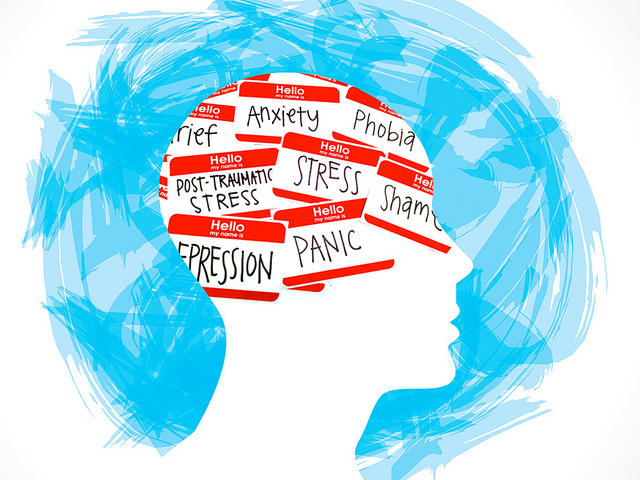
\includegraphics[scale=0.5]{paper/depress_detect.jpeg} 
\shorthandoff{=}
\end{figure}

\newpage

\tableofcontents

\newpage




\section{Background/Summary of the Proposal}

Recent research by WHO suggests that in the world, more than 264 million suffer from depression. Early intervention proved to be efficient in preventing severe depression. However, there are 2 main problems that make early intervention, or any intervention at all, harder to materialize. First of all, intervention requires ever presence of a certified individual in the relevant space. For instance, if the case is child depression, then a psychiatrist needs to be present in the school on a regular basis. Secondly, the fear of public judgement might prevent individuals to seek help from a person or express what they feel completely. In light of these problems, having an automated system that eliminates the necessity of a certified individual and removes the human judgement factor becomes a necessity. Moreover, such a system can suggest a psychiatrist an early diagnose, which then they can use to build on. Therefore, we seek to build a deep learning model that can identify early indications of human depression using a series of interviews conducted. Our contribution to the literature will be the identification of questions that possesses more valuable information in terms of identifying depression.  

\section{Goal and Objectives}

We are planning to build a detection model that is comparable with the literature. In that sense, our first step is to build a generic model that can classify depression, and present that in mid-quarter presentations. Then, we will move on to our unique contribution which will be evaluating question importance which will be used to present our final findings at the end of the quarter.

Our goal is to use PyTorch and TensorFlow libraries as we learn more about them in class. We will be also building different models (RNN, LSTM, bi-LSTM) and comparing their performances. We will evaluate our work using several pre made models for this problem. Since there's no way of bench-marking question importance identification, as we believe it has not been done before, we will be comparing the performance of different models for this analysis. Our final goal is to test the model using different data-sets (if we can find other, equally comprehensive data) and see if the result is persistent amongst different trained models.

\section{Data}

The DAIC-WoZ Depression Database is part of a larger corpus, the Distress Analysis Interview Corpus (DAIC) (Gratch et al.,2014), that contains clinical interviews designed to support the diagnosis of psychological distress conditions such as anxiety, depression, and post-traumatic stress disorder. These interviews were collected as part of a larger effort to create a computer agent that interviews people and identifies verbal and nonverbal indicators of mental illness (DeVault et al., 2014). Data collected include audio and video recordings and extensive questionnaire responses; this part of the corpus includes the Wizard-of- Oz interviews, conducted by an animated virtual interviewer called Ellie, controlled by a human interviewer in another room. Data has been transcribed and annotated for a variety of verbal and non-verbal features. This data includes 189 sessions of interactions ranging between 7-33 minutes (average is 16 minutes). Each session includes transcripts of the interaction, participant audio files, and information about facial features.



\section{Related Work}

Because the DAIC-WoZ Depression Database is one of only two public-use depression databases of its kind, there is a wide literature on the analysis of this data, both from a computational perspective as well as qualitatively. In particular, some of the related work we plan to use as inspiration is:

\begin{itemize}
    \item Lin L, Chen X, Shen Y, Zhang L. Towards Automatic Depression Detection: A BiLSTM/1D CNN-Based Model. Applied Sciences. 2020; 10(23):8701. 
    \item Cohn, J.F.; Kruez, T.S.; Matthews, I.; Yang, Y.; Nguyen, M.H.; Padilla, M.T.; Zhou, F.; De La Torre, F. Detecting depression from facial actions and vocal prosody. In Proceedings of the 2009 3rd International Conference on Affective Computing and Intelligent Interaction and Workshops.
    \item Meng, H.; Huang, D.; Wang, H.; Yang, H.; AI-Shuraifi, M.; Wang, Y. Depression Recognition Based on Dynamic Facial and Vocal Expression Features Using Partial Least Square Regression. In Proceedings of the 3rd ACM international workshop on Audio/visual emotion challenge.
\end{itemize}





Lin et al. uses a bi-LSTM model with an attention layer and process audio & text features. They use ELMO word embeddings to create an embedding layer for the input text. One thing they note is the imbalance of the data between depressed and non depressed individuals. Therefore, they use a data re-sampling method to balance out two subclasses. They group every 10 response of a depressed individual, then they randomly select one response from the group. This process will be replicated in our project as well. They used traditional model testing metrics, F1 score, Recall, Precision. They also used a simple regression model to compare their results. The metrics they used are MAE and RMSE.

\begin{figure}[h!]
\centering
\caption{Sample Results from Li et al.}\label{PG_A1}
\shorthandoff{=}
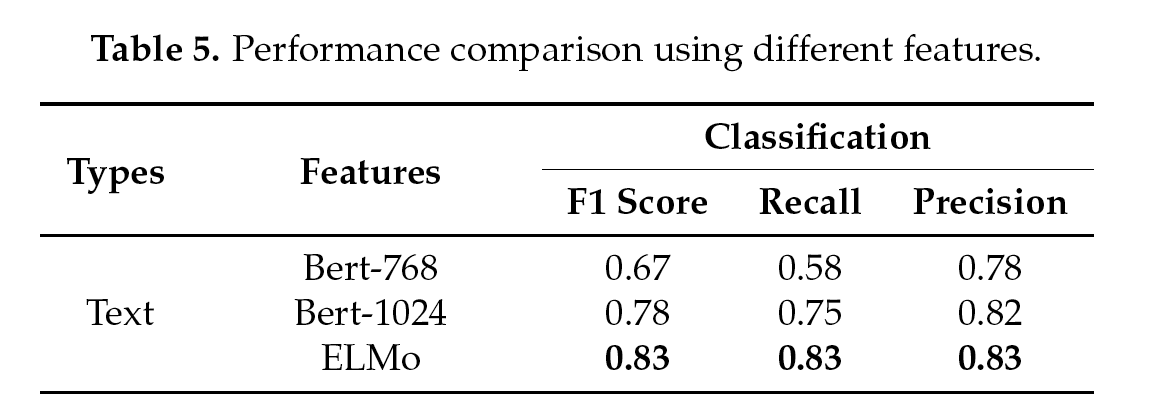
\includegraphics[scale=0.5]{paper/sample_results.png} 
\shorthandoff{=}
\end{figure}


It appears that their results with ELMO embeddings are much better than pre-trained BERT embeddings. We will also compare different embeddings and models to have such a result.



\newpage

\section{Work Split}

In the beginning of the project we are going to be doing a lot of coding together on the same tasks as we figure out how best to work with all of the elements of this data. After we get the initial data processed and ready to feed to a model, one of us will write the code to create the model and the other person will work with the model to see if it is possible to accurately detect depression in an abridged version of the transcripts. 